%revetement, revetement universel, correspondance de Galois

\section{Revêtement, deuxième partie}

Nous avons introduit dans la partie \ref{covering-space-intro} la notion de revêtement, et ensuite vu comment elle pouvait nous aider à calculer le groupe fondamental du cercle. En réalité, la théorie sur les revêtements est bien plus profonde que cela, avec en autre un fort attachement à l'algèbre, avec une correspondance de Galois.

\subsection{Correspondance de Galois}

Tout d'abord, il faut comprendre qu'un espace ne possède pas qu'un seul revêtement. Avec l'exemple du cercle, nous avons choisi, lors du calcul du groupe fondamental \ref{th:grp-funda-circle}, la droite réelle, mais il en existe bien d'autres. Rien n'empêche le revêtement de faire deux tours au dessus du cercle, pour revenir au point de départ.
\begin{figure}[H]
\centering
\begin{subfigure}[b]{0.45\linewidth}
\centering
    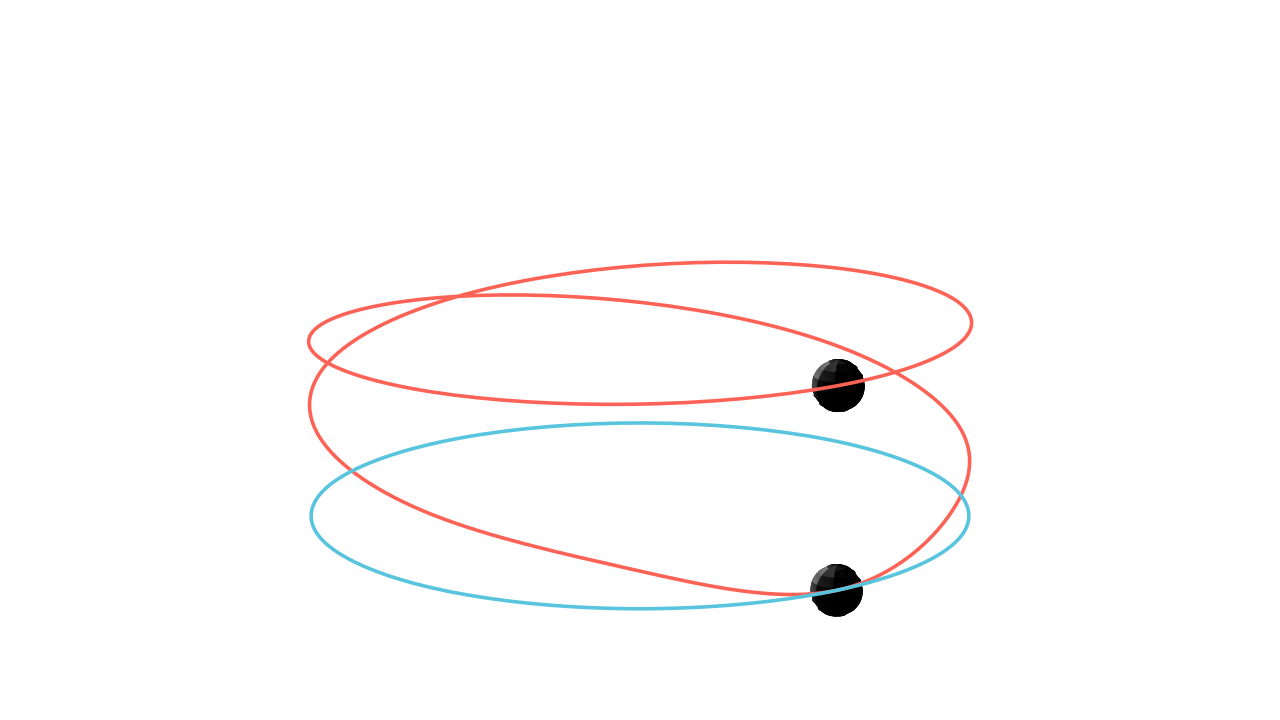
\includegraphics[width=.8\linewidth]{pictures/CoverCircle2_ManimCE_v0.18.1.png}
    \caption{\centering Exemple de revêtement (rouge) pour le cercle (bleu)}
    \label{fig:cover-circle-2}
\end{subfigure}
\hspace{5pt}
\begin{subfigure}[b]{0.45\linewidth}
\centering
    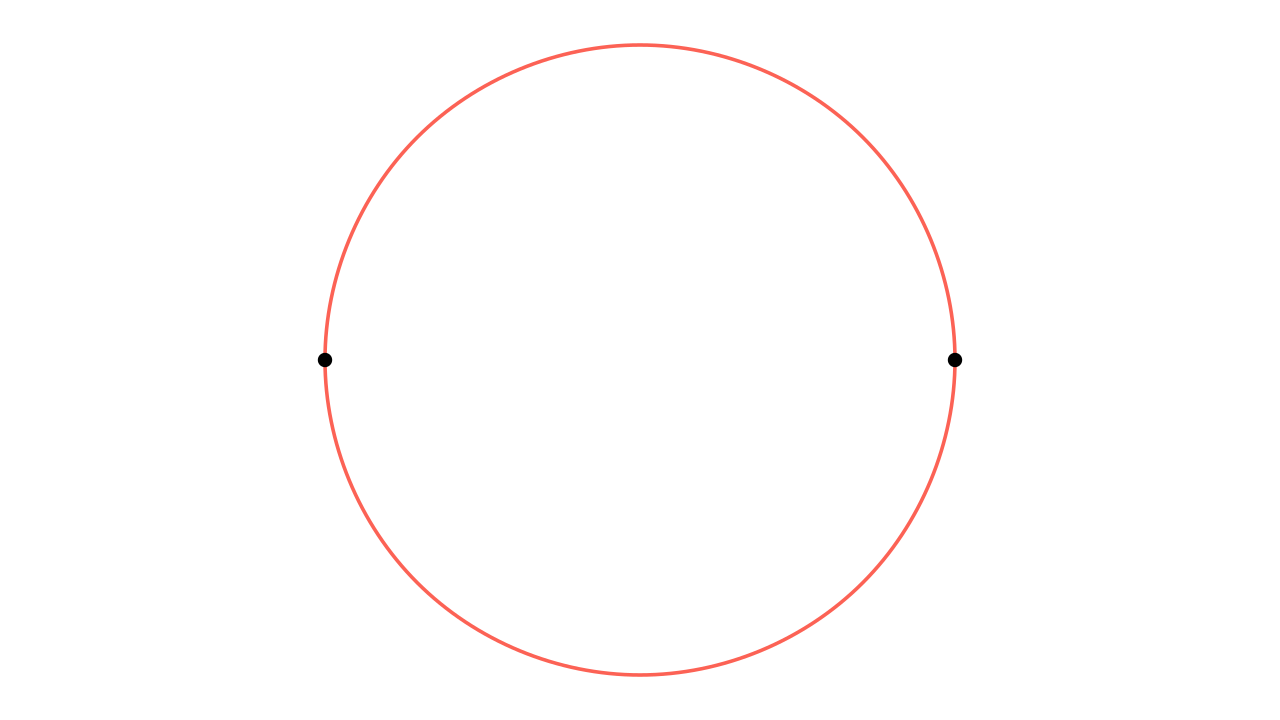
\includegraphics[width=.8\linewidth]{pictures/CoverCircle2_3_ManimCE_v0.18.1.png}
    \caption{\centering Revêtement vu comme un cercle, 2 fois plus long que l'original}
    \label{fig:cover-circle-2-2}
\end{subfigure}
\end{figure}

Pour cet exemple, nous pouvons supposer qu'il existe autant de revêtements qu'il existe d'entiers naturels... mais comment le démontrer ? C'est ce que nous allons voir par la suite.

\subsubsection{Énonce du théorème}

\begin{definition}
Un espace $X$ est \emph{localement connexe par arc} si pour tout voisinage de~$x\in X$, il existe un voisinage inclut dans le premier tel que celui-ci est connexe par arc.

Un espace est dit \emph{semi-localement simplement connexe} si pour tout voisinage de tout point $x\in X$, les lacets dans ce voisinage sont homotopes au lacet constant une fois plongés dans $X$. Autrement dit, le groupe fondamental du voisinage devient trivial dans $X$.
\end{definition}

\begin{exemple}
Un espace avec deux composantes connexes par arc disjointes est localement connexe par arc : il suffit de prendre un voisinage se trouvant dans une seule des deux composantes.

Tout espace simplement connexe est semi-localement simplement connexe. Par exemple, avec~${X=D^2}$, si l'on prend un voisinage étant homéomorphe à une couronne (ie. il possède un trou), son groupe fondamental est certes non trivial, mais une fois plongé dans l'espace $X$, les classes d'homotopies sont toutes égales à celle du lacet constant.
\end{exemple}

Un morphisme entre deux revêtements $p_1:\Tilde{X}_1\to X$ et $p_2:\Tilde{X}_2\to X$ est une application~${f:\Tilde{X}_1\to\Tilde{X}_2}$, amenant un point de base $\Tilde{x}_1\in p_1\inv(x_0)$ vers un point de base $\Tilde{x}_2\in p_2\inv(x_0)$.

\begin{theorem}
Pour un espace pointé $(X,x_0)$ connexe par arc, localement connexe par arc, et semi-localement simplement connexe, il existe une bijection entre :\begin{itemize}
    \item les sous groupes de $\pi_1(X,x_0)$ ;
    \item les revêtements $p:(\Tilde{X},\Tilde{x}_0)\to(X,x_0)$, à isomorphisme près de revêtements, conservant le point de base ;
\end{itemize} obtenue en associant le groupe $p_\ast(\pi_1(\Tilde{X},\Tilde{x}_0))$ au revêtement $(\Tilde{X},\Tilde{x}_0)$.
\end{theorem}

Pour la démonstration nous allons tout d'abord montrer que le morphisme induit $p_\ast$ est injectif, puis nous allons construire le revêtement lié au sous groupe trivial. Par la suite, nous montrerons que nous pourrons associer un revêtement à un sous groupe du groupe fondamental, pour enfin voir que les classes d'isomorphismes de revêtements induisent le même morphisme.

\subsubsection{Démonstration}

Nous considérons au cours de cette partie un espace pointé $(X,x_0)$ connexe par arc, localement connexe par arc, et semi-localement simplement connexe.

\begin{proposition}
Pour un revêtement $p:(\Tilde{X},\Tilde{x}_0)\to(X,x_0)$, le morphisme induit $p_\ast$ est injectif.
\end{proposition}
\begin{proof}
Le morphisme $p_\ast$ envoie $[\Tilde{\gamma}]\in\pi_1(\Tilde{X},\Tilde{x}_0)$ vers $[p\Tilde{\gamma}]\in\pi_1(X,x_0)$. Soit $[\Tilde{\gamma}]\in\ker(p_\ast)$, c'est à dire que $p\Tilde{\gamma}$ est homotope au lacet constant. Par relèvement d'homotopie, le lacet $\Tilde{\gamma}$ est homotope au lacet constant dans $(\Tilde{X},\Tilde{x}_0)$.
\end{proof}

\begin{definition}
Un revêtement simplement connexe est appelé \emph{revêtement universel}, et comme il est unique à isomorphisme près avec la correspondance de Galois, nous l'appelons le revêtement universel.
\end{definition}

\begin{proposition}
Pour $X$ un espace connexe par arc, localement connexe par arc, et semi-localement simplement connexe, il existe un revêtement universel.
\end{proposition}
La démonstration se fait par construction du revêtement et d'une topologie adéquate. Pour définir une topologie sur le revêtement, nous allons construire une base de topologie.

\begin{definition}
Une \emph{base de topologie} sur un ensemble $Y$ est une collection $\mathcal{B}$ telle que :\begin{enumerate}
    \item $Y=\bigcup_{V\in B}V$ ;
    \item Pour $U,U'\in \mathcal{B}$ et $y\in U\cap U'$, il existe un $V\in\mathcal{B}$ tel que $y\in V\subseteq U\cap U'$.
\end{enumerate}
En notant $\mathcal{T}$ l'ensemble des des sous-ensembles de $Y$ pouvant être écrit comme union d'éléments de~$\mathcal{B}$, alors $\mathcal{T}$ est une topologie de $Y$.
\end{definition}
Nous pouvons désormais commencer la démonstration.
\begin{proof}
Nous considérons l'ensemble $\Tilde{X}=\{[\gamma],\gamma\text{ chemin de $X$, $\gamma(0)=x_0$}\}$ et l'application~${p:\Tilde{X}\to X, [\gamma]\mapsto\gamma(1)}$. Nous allons montrer que le couple $(\Tilde{X},p)$ est un revêtement de $X$ simplement connexe.

L'application $p$ est bien définie, puisque pour $\gamma\simeq\gamma'$, nous avons les extrémités qui sont conservées. De plus, l'application est surjective puisque $X$ est connexe par arc.

\bigskip Pour définir une base de topologie sur $\Tilde{X}$, nous allons commencer par en trouver une adéquate pour $X$. Ensuite nous allons montrer qu'avec cette base, la projection définie un revêtement, notamment avec l'image réciproque qui est une union disjointe d'ouvert de $\Tilde{X}$. Enfin, nous montrerons que ces ouverts forment une base de topologie sur $\Tilde{X}$.

Tout d'abord, comme $X$ est un espace localement connexe par arc et semi-localement simplement connexe, l'ensemble des ouverts connexes par arc tel que leurs groupes fondamentaux sont triviaux dans $X$ forme un recouvrement, que l'on note : \[B_X=\{U\subset X \text{ouvert connexe par arc et } i_\ast(\pi_1(U))=1\in\pi_1(X)\}.\]Montrons que ceci forme une base de topologie de $X$. Soient deux ouverts $U,U'\in\mathcal{B}_X$, et soit un point $x\in U\cap U'$. Par la connexité parc arc locale, nous savons qu'il existe $V\subseteq U\cap U'$ tel que $V$ soit connexe par arc. De plus, puisque $V\subset U$, nous avons la chaîne d'inclusion $V\hookrightarrow U\hookrightarrow X$ qui induit un morphisme sur les groupes fondamentaux. Comme $\pi_1(U)\mapsto 1\in \pi_1(X)$, il en est de même pour~$V$. Nous en déduisons alors que $V\in \mathcal{B}_X$. Nous pouvons ainsi conclure que l'ensemble $\mathcal{B}_X$ forme une base de topologie de $X$.

Soit $U_i\in\mathcal{B}_X$. Étant donné que son groupe fondamental est trivial dans $X$, chaque classe d'homotopie de chemins est uniquement déterminée par ses extrémités. Si l'on fixe le point de départ, à~$x_0$ par exemple, nous obtenons ainsi une union disjointe :$$p\inv(U_i)=\bigsqcup_{x\in U_i}\{[\gamma],\gamma\text{ chemin de $U_i$ tel que }\gamma(0)=x_0,\gamma(1)=x\}.$$Cet union est bien trop gros et ne peut formé une base de topologie sur $\Tilde{X}$. Nous définissons alors une relation sur les classes d'homotopies de chemins : $[\gamma]\approx[\gamma']$ si et seulement s'il existe $\eta$ un chemin de~$U_i$ tel que $\gamma\cdot\eta=\gamma'$. Il n'est pas difficile de vérifier que cette relation est une relation d'équivalence. Nous noterons $V_{ij}$ l'ensemble des classes d'équivalences de $\approx$ sur $U_i$, indexé par $j$. Nous obtenons alors une union disjointe avec ces ensembles : \[p\inv(U_i)=\bigsqcup_{j}V_{ij}=\bigsqcup_j\{[\gamma\cdot\eta],\eta\text{ chemin de $U_i$ avec $\eta(0)=\gamma(1)$}\}.\]Soit $V_{ij}\in p\inv(U_i)$. Montrons que $p:V_{ij}\to U_i$ est une bijection. Il est clair que l'application est surjective, puisque $U_i$ est connexe par arc. Pour montrer qu'elle est injective, supposons que l'on ait~$p([\gamma\cdot\eta])=p([\gamma'\cdot\eta'])$. Par définition de $p$, nous avons $\eta(1)=\eta'(1)$. Par simple connexité semi locale, les deux chemins $\gamma\cdot\eta$ et $\gamma'\cdot\eta'$ sont homotopes, car possède les mêmes extrémités. Autrement dit, nous avons $[\gamma\cdot\eta]=[\gamma'\cdot\eta']$, ce qui fait de $p$ une application injective.

Il reste à démontrer que les $V_{ij}$ forment une base de topologie de $\Tilde{X}$. Nous noterons cet ensemble ainsi : $$\mathcal{B}_{\Tilde{X}}=\bigcup_ip\inv(U_i)=\bigcup_{i,j}V_{ij}.$$ Il est clair que cela forme un recouvrement de $\Tilde{X}$. Soit $V_{ij},V_{i'j'}\in\mathcal{B}_{\Tilde{X}}$ deux ouverts de cet ensemble, avec $\Tilde{x}\in V_{ij}\cap V_{i'j'}$. Il existe, par définition de la base de topologie de $X$, un ouvert $U\in \mathcal{B}_X$ tel que~${p(y)\in U\subset U_i\cap U_{i'}=p(V_{ij})\cap p(V_{i'j'})}$. Par définition, la relation d'équivalence sur $U$ implique la relation sur $U_i$ et $U_j$. Ainsi, la classe d'équivalence $V\in p\inv(U)$ contenant $y$ vérifie $V\subset V_{ij}\cap V_{i'j'}$. Ainsi, nous avons montré que $B_{\Tilde{X}}$ est une base de topologie sur $\Tilde{X}$. Il est assez facile de voir qu'avec ces bases de topologie, $p:\Tilde{X}\to X$ est un revêtement : l'image réciproque de tout ouvert de $\mathcal{B}_X$ est dans $\mathcal{B}_{\Tilde{X}}$ (continuité de $p$), et toute image d'ouvert de $\mathcal{B}_{\Tilde{X}}$ est un ouvert de $\mathcal{B}_X$ (montrant la continuité de la réciproque, et donc l'homéomorphisme $p:V_{ij}\to U_i$).

\bigskip Il nous reste alors plus qu'à montrer la simple connexité de $\Tilde{X}$. Tout d'abord, nous pouvons remarquer que $\Tilde{X}$ est connexe par arc, puisqu'il existe un chemin entre $[x_0]$, le chemin constant basé en $x_0$, et $[\gamma]\in \Tilde{X}$ : il suffit de prendre le chemin~$[\gamma|_{[0,t]}], t\in[0,1]$. Pour la simple connexité, on considère un lacet~$f$ de $\Tilde{X}$ basé en $[x_0]$, et on note $pf=\gamma$, un lacet basé en $x_0$. Si on note le chemin $\gamma_t=~\gamma|_{[0,t]}$, de telle sorte que $[\gamma_t]$ est un relèvement de $\gamma$, nous avons~$[\gamma_0]=[x_0]=f(0)$. Par unicité du relèvement, nous obtenons $[\gamma_t]=f(t)$, et en particulier l'égalité~$[\gamma_1]=f(1)=[x_0]$. Comme $\gamma_1=\gamma$, on en déduit $[\gamma]=[x_0]$ : la projection $pf=\gamma$ est homotope au lacet constant. Par injectivité de $p_\ast$, nous avons~$p_\ast([f])=0$ qui implique $[f]=0$, d'où le fait que $\Tilde{X}$ soit simplement connexe.
\end{proof}

Cette construction théorique est efficace car elle permet d'affirmer l'existence du revêtement universel pour un espace vérifiant les propriétés demandées. De plus, elle permet de démontrer d'autres résultats théoriques, comme la proposition qui suit. En revanche, lors de calculs concrets, ce n'est pas cette méthode qui est utilisée (il suffit de voir le revêtement universel du cercle).

\begin{proposition}
Soit $X$ un espace connexe par arc, localement connexe par arc, et semi-localement simplement connexe. Pour chaque $H$ sous groupe de~$\pi_1(X,x_0)$, il existe un revêtement~${p:X_H\to X}$, tel que $p_\ast(\pi_1(X_H,\Tilde{x}_0))=H$, pour un certain $\Tilde{x}_0\in X_H$.
\end{proposition}
\begin{proof}
On définit tout d'abord une relation sur le revêtement universel $\Tilde{X}$ de~$X$ : \[[\gamma]\approx[\gamma']\Longleftrightarrow\gamma(1)=\gamma'(1)\text{ et }[\gamma\cdot\overline{\gamma'}]\in H.\]Il est facile de voir qu'il s'agit d'une relation d'équivalence, nous allons pouvoir passer au quotient et définir $p:X_H\to X$ avec $X_H=X/\approx$.

Nous choisissons comme point de base $\Tilde{x}_0\in X_H$, la classe d'équivalence du chemin constant~$c$ en~$x_0$. Montrons que $p_\ast(\pi_1(X_H,\Tilde{x}_0))=H$. Étant donné un lacet $\gamma$ de $(X,x_0)$, il se relève en un chemin de $[c]$ vers $[\gamma]$. Pour que l'image du relèvement de $\gamma$ sur $X_H$ soit un lacet, il faut que~$[\gamma]\approx[c]$. Autrement dit, il faut que $[\gamma]\in H$.
\end{proof}

Il nous reste à démontrer que les revêtements correspondant à un même sous-groupe sont identiques, à isomorphisme près.

\begin{proposition}
Soit $X$ un espace connexe par arc, localement connexe par arc, et semi-localement simplement connexe. Deux revêtements sont isomorphes si et seulement si les sous-groupes induits par l'image du morphisme induit par leurs projections sont identiques.
\end{proposition}

\begin{proof}
Soient $p_1:(\Tilde{X}_1,\Tilde{x}_1)\to (X,x_0)$ et $p_2:(\Tilde{X}_2,\Tilde{x}_2)\to (X,x_0)$, avec~$\Tilde{x}_1\in p_1\inv(x_0)$ et~${\Tilde{x}_2\in p_2\inv(x_0)}$. Montrons que ces revêtements sont isomorphes ssi ${p_{1\ast}(\pi_1(\Tilde{X}_1,\Tilde{x}_1))=p_{2\ast}(\pi_1(\Tilde{X}_2,\Tilde{x}_2)}$.

Supposons que les revêtements soient isomorphes via $f:\Tilde{X}_1\to \Tilde{X}_2$. Nous avons alors les égalités~${p_1=p_2f}$ et $p_2=p_1f\inv$. L'application $f$ induit un isomorphisme $f_\ast:\pi_1(\Tilde{X}_1,\Tilde{x}_1)\to \pi_1(\Tilde{X}_2,\Tilde{x}_2)$, de telle sorte que $p_{1\ast}f_\ast=p_{2\ast}$ et $p_{2\ast}f\inv_\ast=p_{1\ast}$, ce qui nous donne : \[p_{2\ast}(\pi_1(\Tilde{X}_2,\Tilde{x}_2))=p_{1\ast}f_\ast(\pi_1(\Tilde{X}_2,\Tilde{x}_2))=p_{1\ast}(\pi_1(\Tilde{X}_1,\Tilde{x}_1)),\] ainsi que \[p_{1\ast}(\pi_1(\Tilde{X}_1,\Tilde{x}_1))=p_{2\ast}f\inv_\ast(\pi_1(\Tilde{X}_1,\Tilde{x}_1))=p_{2\ast}(\pi_1(\Tilde{X}_2,\Tilde{x}_2)).\]

Supposons désormais que les sous-groupes induits sont identiques. Par le critère de relèvement, il existe $\Tilde{p}_1:(\Tilde{X}_1,\Tilde{x}_1)\to(\Tilde{X}_2,\Tilde{x}_2)$, tel que $p_2\Tilde{p}_1=p_1$. De même, il existe $\Tilde{p}_2:(\Tilde{X}_2,\Tilde{x}_2)\to(\Tilde{X}_1,\Tilde{x}_1)$, avec $p_1\Tilde{p}_2=p_2$. Par unicité du relèvement, nous avons $\Tilde{p}_1\Tilde{p}_2=id$ et $\Tilde{p}_2\Tilde{p}_1=id$, ce qui fait de $\Tilde{p}_1$ et $\Tilde{p}_2$ des isomorphismes.
\end{proof}

Finalement, avec ces trois propositions, nous avons toutes les cartes pour démontrer le théorème.

\bigskip Néanmoins, il reste un fait algébrique intéressant, renforcant le lien de la correspondance de Galois.

\begin{proposition}
Soit $X$ un espace, et $(\Tilde{X},p)$ un revêtement de $X$. On appelle \emph{fibre}, ou feuillet, de $x_0\in X$, un élément de $p\inv(x_0)$. Le nombre de fibres est constant pour tout $x_0\in X$, et est égal à l'indice du sous groupe $p_\ast(\pi_1(\Tilde{X},\Tilde{x}_0))$, avec $\Tilde{x}_0\in p\inv(x_0)$.
\end{proposition}

L'idée de la démonstration est de montrer que pour tout élément du recouvrement $U_i\in X$, le cardinal de $p\inv (U_i)$ ne dépend pas du choix de $U_i$. Cela vient du fait que les $U_i$ peuvent se chevaucher, ayant alors le même cardinal pour l'image réciproque.

\begin{exemple}
Reprenons l'exemple du cercle. Son revêtement universel est celui dont nous nous sommes servi pour la démonstration, à savoir $\bb{R}$, puisqu'il est simplement connexe. Avec la dernière proposition et le théorème, nous pouvons déduire que le revêtement avec $n$ feuillets est en bijection avec le sous-groupe $n\bb{Z}$ dans $\pi_1(\s{1},(1,0))$, car $[\bb{Z}:n\bb{Z}]=|\bb{Z}_n|=n$.
\end{exemple}

\subsection{Transformation de deck}

Pour un revêtement $p:\Tilde{X}\to X$, on appelle \emph{transformation de deck}, ou transformation de revêtement, tout isomorphisme $\Tilde{X}\to\Tilde{X}$. Il est important de voir que pour conserver la structure du revêtement, toute les opérations sur un espace (comme les symétries) ne sont pas autorisées. La transformation doit en autres conserver l'ordre des feuillets (voir figure \ref{fig:deck-transformation}). De ce fait, et de la propriété d'unicité du relèvement, la transformation est entièrement déterminée par la transformation d'un point (les autres suivront la même transformation).

\begin{figure}[H]
    \centering
    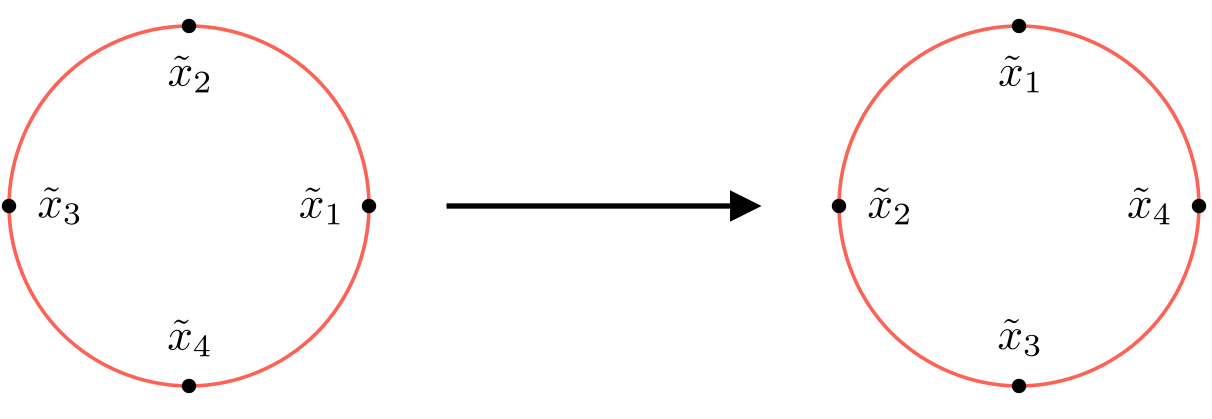
\includegraphics[width=0.5\linewidth]{pictures/CoverCircle2_2_ManimCE_v0.18.1.png}
    \caption{Exemple de transformation de deck}
    \label{fig:deck-transformation}
\end{figure}

L'ensemble des transformations de deck d'un revêtement $\Tilde{X}$, noté généralement $G(\Tilde{X})$, possède en réalité une structure de groupe. Muni de la composition d'isomorphismes, il est clair que l'élément neutre est l'application l'identité, que les transformations admettent un symétrique, et que la loi est associative. 

De plus, on dit qu'un revêtement est \emph{normal} si pour tout $x\in X$, tout couple~$(\Tilde{x},\Tilde{x}')\in p\inv(x)$, il existe une transformation passant de~$(\Tilde{X},\Tilde{x})$ à $(\Tilde{X},\Tilde{x}')$.

\begin{exemple}
Pour un revêtement du cercle à $n$ feuillets, les transformations de deck sont les isomorphisme $\varphi_k:z\mapsto z^k$ pour $k\in\bb{Z}^*$. Nous pouvons remarquer que l'on a $\varphi_k=\varphi_{an+k}$, pour $a$ entier. D'où la conjecture du fait que~$G(\Tilde{X})\cong\bb{Z}_n$.
\end{exemple}

Les transformations de deck ont un lien très étroit avec la correspondance de Galois, comme peut nous le montrer la proposition qui suit : 

\begin{proposition}
Soit $p:(\Tilde{X},\Tilde{x}_0)\to(X,x_0)$ un revêtement connexe par arc d'un espace $X$ connexe par arc et localement connexe par arc. En notant le sous-groupe $H=p_\ast(\pi_1(\Tilde{X},\Tilde{x}_0))$ de~$\pi_1(X,x_0)$, nous avons : \begin{itemize}
    \item Le revêtement est normal si et seulement si $H$ est un sous-groupe normal ;
    \item Le groupe $G(\Tilde{X})$ est isomorphe à $N(H)/H$, où $N(H)$ est le normalisateur.
\end{itemize}
En particulier, si $\Tilde{X}$ est un revêtement normal, alors $G(\Tilde{X})\cong \pi_1(X,x_0)/H$.
\end{proposition}

\textbf{[insérer preuve]}

Les transformations de deck sont un cas particulier de ce que l'on appelle une action de groupe sur un espace.

\begin{definition}\label{def:group-action}
Une action de groupe $G$ sur un espace $X$ est un morphisme $\rho$ de $G$ vers le groupe des homéomorphismes de $X$ dans lui-même, noté~$Homeo(X)$. Ce morphisme est définie pour $g\in G$ par $\rho(g):X\to X$, que l'on simplifiera par $g:X\to X$.
\end{definition}

\begin{remark}
En reprenant les notations de l'énoncé, étant donné que $\rho$ est un morphisme, alors il vérifie $e_G(x)=x$ pour $e_G$ l'élément neutre, pour et $x\in X, g,g'\in G, {g(g'(x))=(gg')(x)}$.
\end{remark}

Il existe également des actions de groupe sur un ensemble quelconque, qui se définissent de manière presque similaire, mais ce ne sont pas ceux qui nous intéresse ici.

\subsubsection{Propriétés sur les actions de groupes}

Une question que l'on pourrait se poser sur les actions de groupes, serait de savoir si elles peuvent représenter des transformations de deck. Il suffirait en effet qu'elles vérifient quelques propriétés pour que ce soit le cas.

\begin{definition}
Étant donné un groupe $G$ et $Y$ un espace, on appelle \emph{orbite} de $y\in Y$ l'ensemble~$Gy=\{g(y),g\in G\}$. L'ensemble des orbites ${Y/G=\{Gy,y\in Y\}}$ est appelé \emph{espace des orbites}
\end{definition}

\begin{exemple}
Pour un revêtement normal, l'espace des orbites $\Tilde{X}/G(\Tilde{X})$ est $X$.
\end{exemple}

Pour une action de groupe $G$ sur l'espace $Y$, notons cette propriété :

\begin{equation}\label{eq:prop-action}
\forall y\in Y,\exists U\in\mathcal{V}(y),\forall g,g'\in G, g(U)\cap g'(U)\neq\emptyset\Longrightarrow g=g'
\end{equation}

Cette propriété est vérifiée par les transformations de deck. De plus, si la propriété est vérifiée, elle permet alors de retomber sur des revêtements. 

\begin{proposition}
Si une action de groupe $G$ sur $Y$ vérifie \eqref{eq:prop-action}, alors :\begin{itemize}
    \item L'application quotient $p:Y\to Y/G$ est un revêtement normal :
    \item Si $Y$ est connexe par arc, alors $G$ est le groupe de transformations de deck du revêtement~${Y\to Y/G}$ ;
    \item Si $Y$ est connexe par arc et localement connexe par arc, alors $G\cong\pi_1(Y/G)/p_\ast(\pi_1(Y))$.
\end{itemize}
\end{proposition}

Une autre question pourrait se poser désormais : quand est-ce qu'une action de groupe vérifie la propriété \eqref{eq:prop-action} ?

\begin{definition}
Une action vérifiant uniquement l'élément neutre comme point fixe est appelée \emph{action libre}.

Une action de groupe $G$ sur $Y$ possède la propriété de \emph{discontinuité propre} si elle vérifie : \[\forall y\in Y,\exists U\in\mathcal{V}(y), |\{g\in G,U\cap g(U)\neq\emptyset\}|<+\infty\]
\end{definition}

\begin{proposition}
Soit $G$ une action de groupe sur $Y$.\begin{itemize}
    \item Si l'action de groupe vérifie \eqref{eq:prop-action}, alors c'est une action libre.
    \item Si $Y$ est Hausdorff, et que l'action est libre et vérifie la discontinuité propre, alors elle vérifie~\eqref{eq:prop-action}.
\end{itemize}
\end{proposition}
\begin{proof}
La première affirmation est évidente.
\end{proof}

\begin{comment}
\begin{proof}
Soit $G$ une action de groupe libre et vérifiant la discontinuité propre sur un espace Hausdorff $Y$. Soit $y\in Y$, et soient deux éléments différents $g,g'\in G$. Notons $y'=g\inv g'(y)$, dont nous savons que $y\neq y'$ du fait que l'action soit libre. Ainsi, le voisinage de $y'$ s'exprime en fonction de celui de $y$. Du fait que l'espace soit Hausdorff, nous savons qu'il existe un ouvert $V\in\mathcal{V}(y)$, avec~$V'=g\inv g'(V)\in\mathcal{V}(y')$, tel que $V\cap V'=V\cap g\inv g'(V)=0$.

Si l'on répète le processus pour tout couples $(g,g')\in G^2$, nous obtenons une famille d'ouvert. Il suffit de prendre l'intersection de ceux-ci pour trouver notre ouvert $U$ vérifiant \eqref{eq:prop-action}.
\end{proof}
\end{comment}

\begin{exemple}
Les actions de groupes finis vérifie la discontinuité propre automatiquement, alors il suffit que ce soit une action libre pour pouvoir vérifier \eqref{eq:prop-action}.
\end{exemple}